\label{sec:unlabelled}

The classification of unlabelled data is completed using the code presented in
Section \ref{sec:q5}. Both implementations are fairly self-explainitory.

The data are clustered and plotted in Figures \ref{fig:k-means-clear},
\ref{fig:k-means-multifuzz} and \ref{fig:k-means-gradientfuzz}. While the
clusters using MCID are essentially the same every time, the clusters from
k-means do not always end up in the same spot and often converge to other
locations. 

As for the multf8 matrix, K-means would likely perform well on that problem
because the data are already clustered by class. Since K-means tries to keep
the class sizes small, it would likely perform well.

\begin{figure}
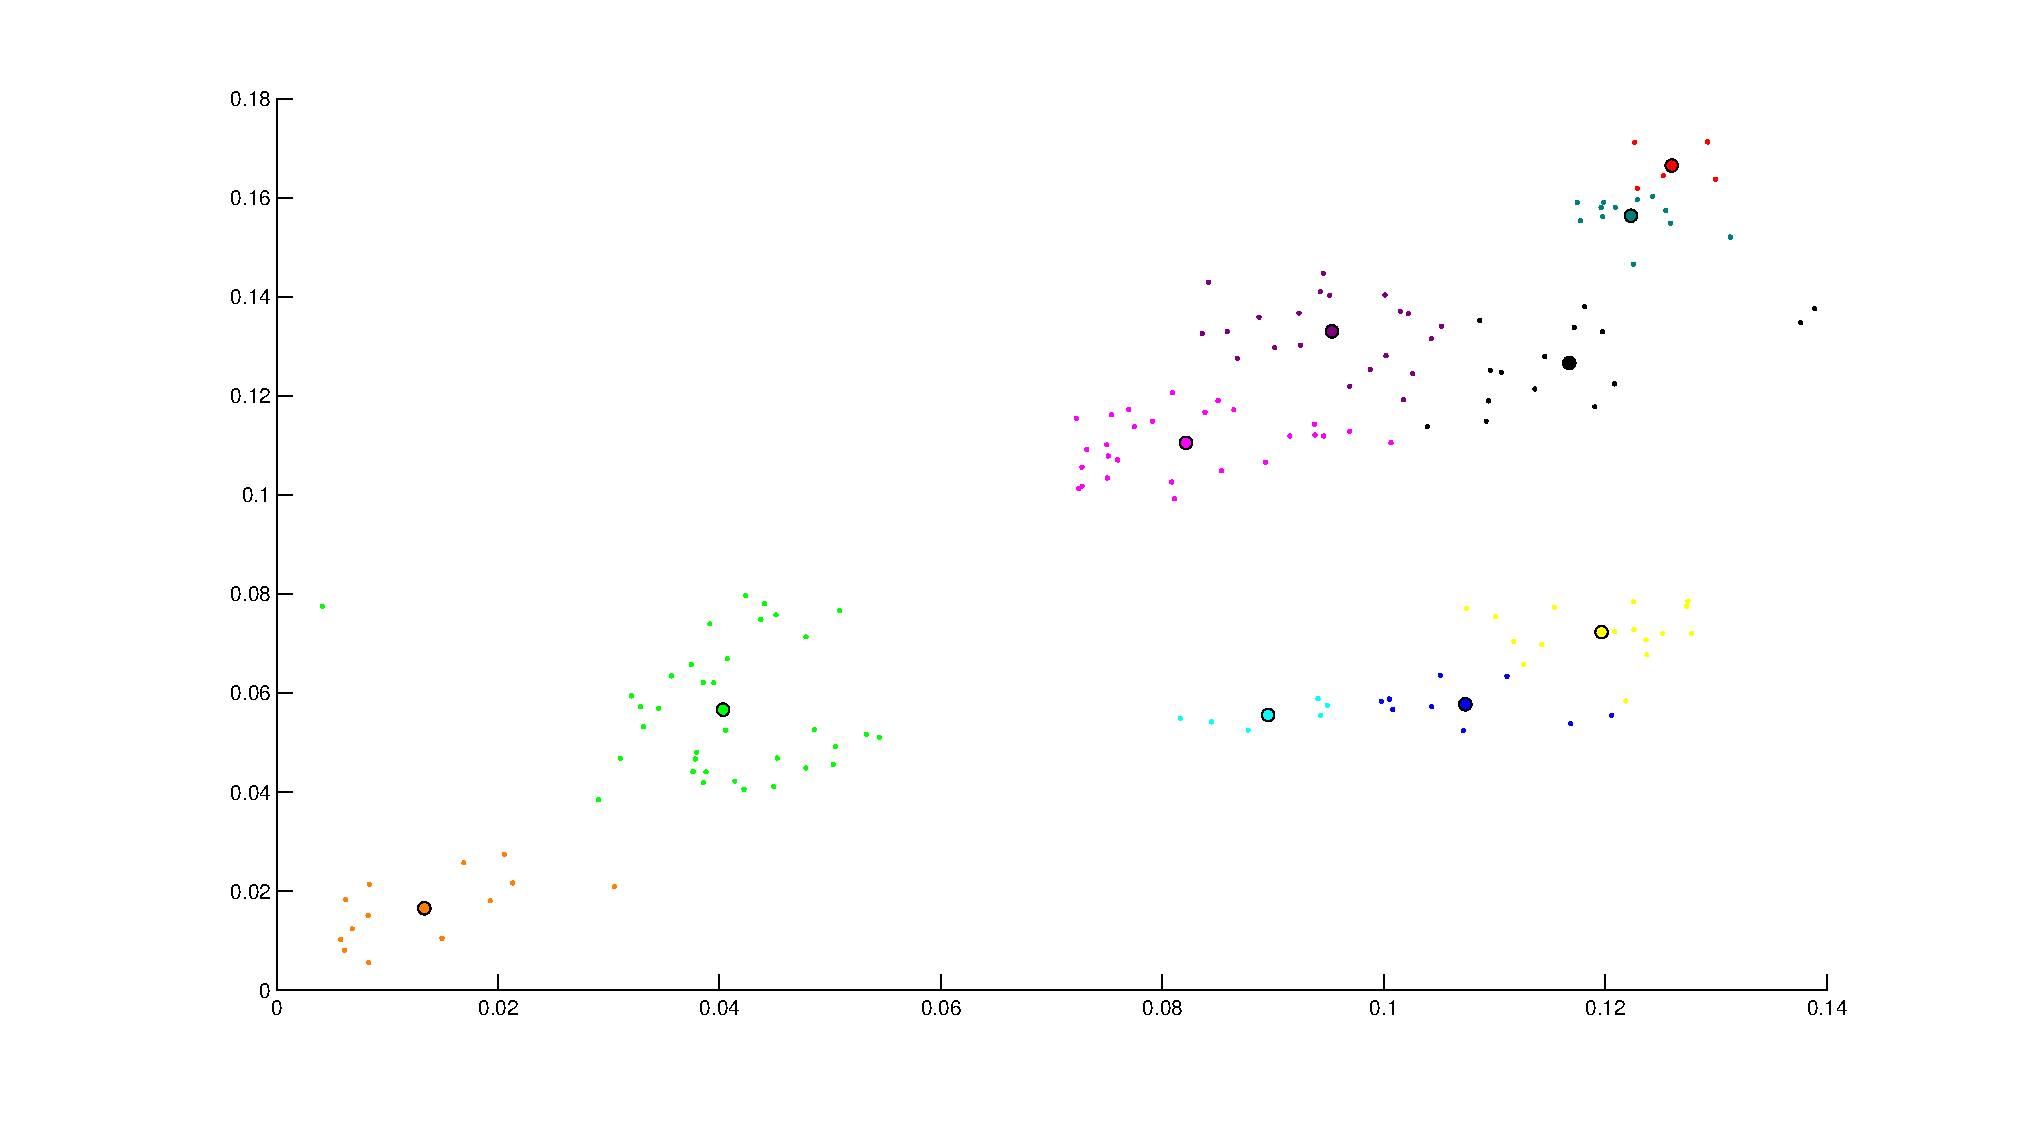
\includegraphics[width=\textwidth]{images/clear-coloured}
\label{fig:k-means-clear}
\caption{K-means clusters, colour-coded with prototypes outlined in black}
\end{figure}

\begin{figure}
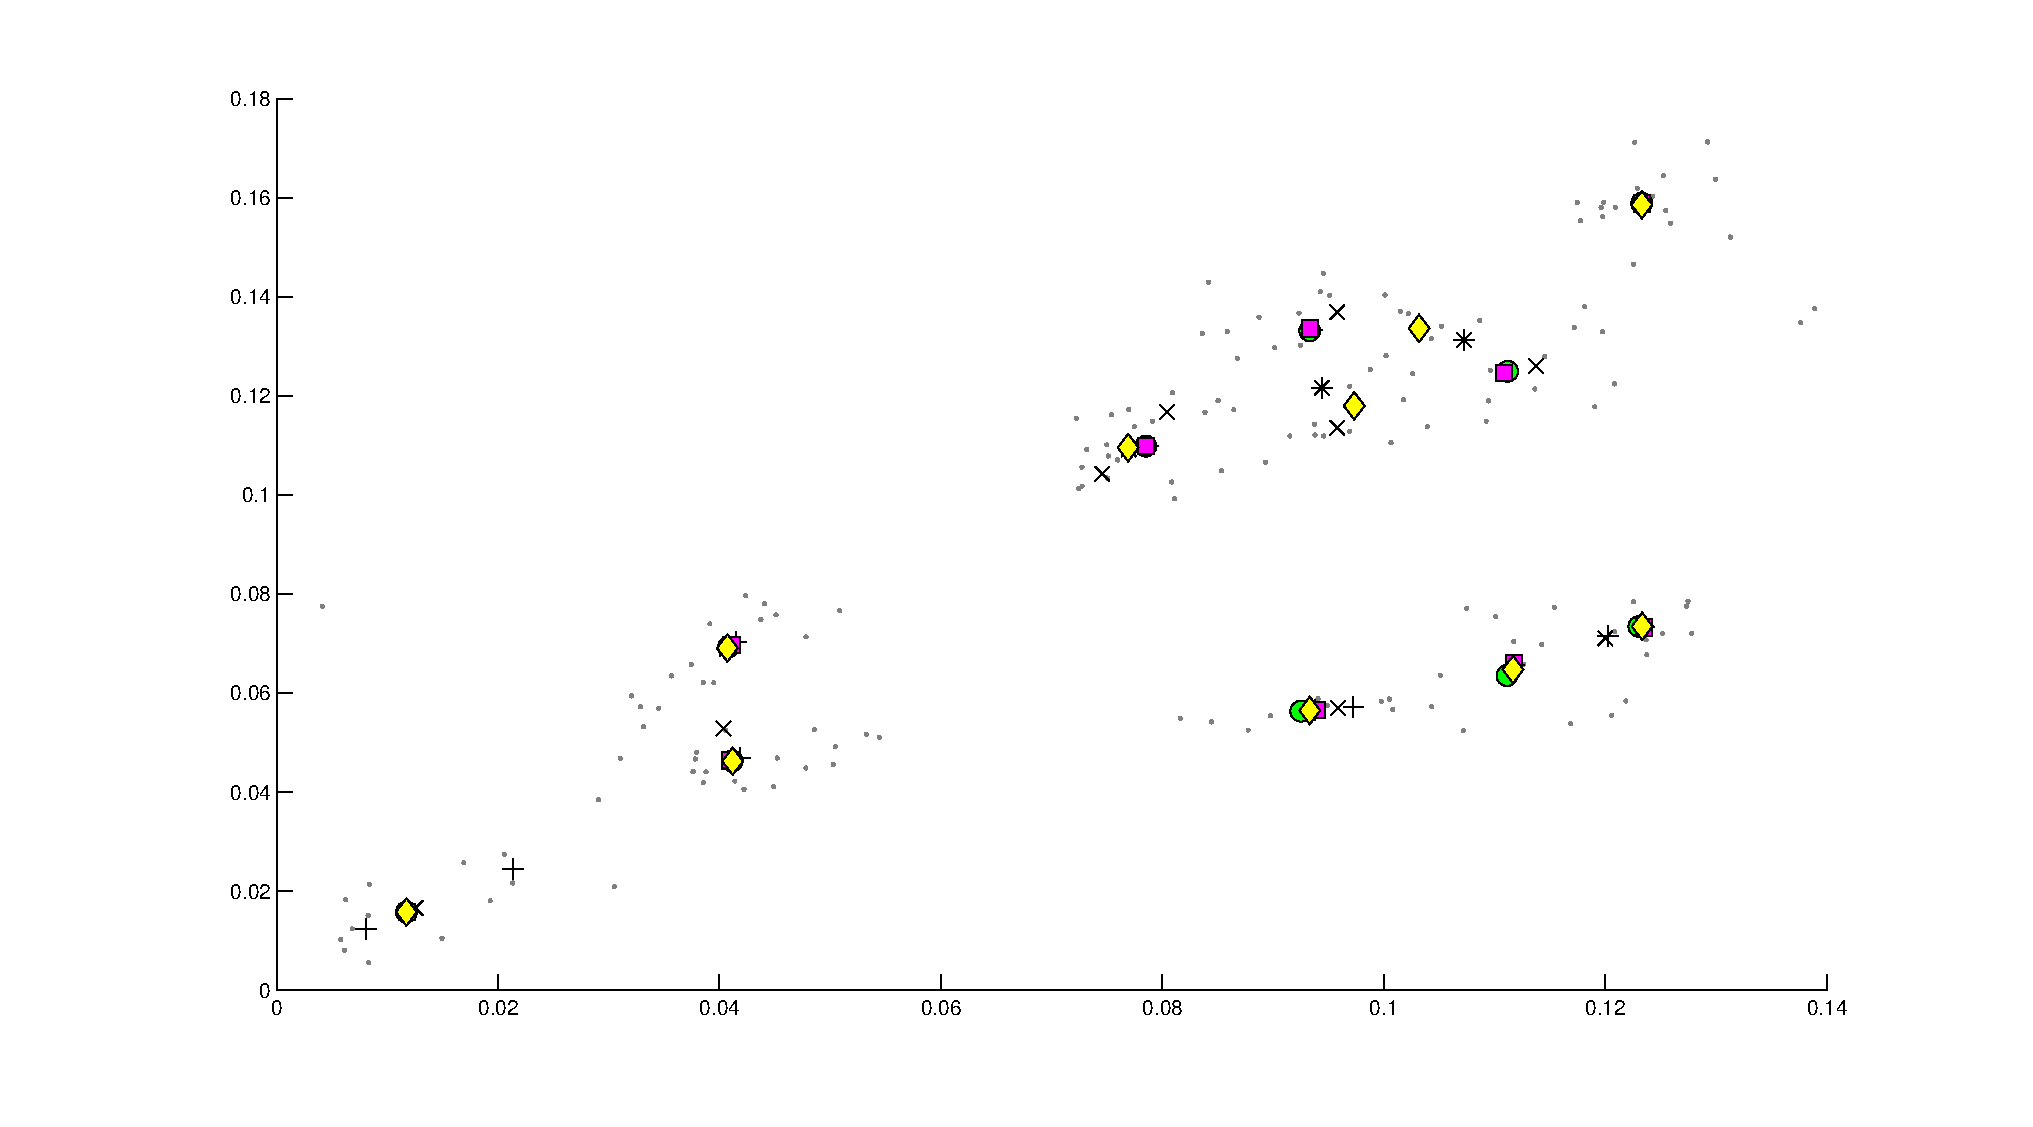
\includegraphics[width=\textwidth]{images/fuzzy-multiple}
\label{fig:k-means-multifuzz}
\caption{Prototypes from multiple runs of the k-means clustering algorithm
(distinct prototype shape and colour for each run)}
\end{figure}

\begin{figure}
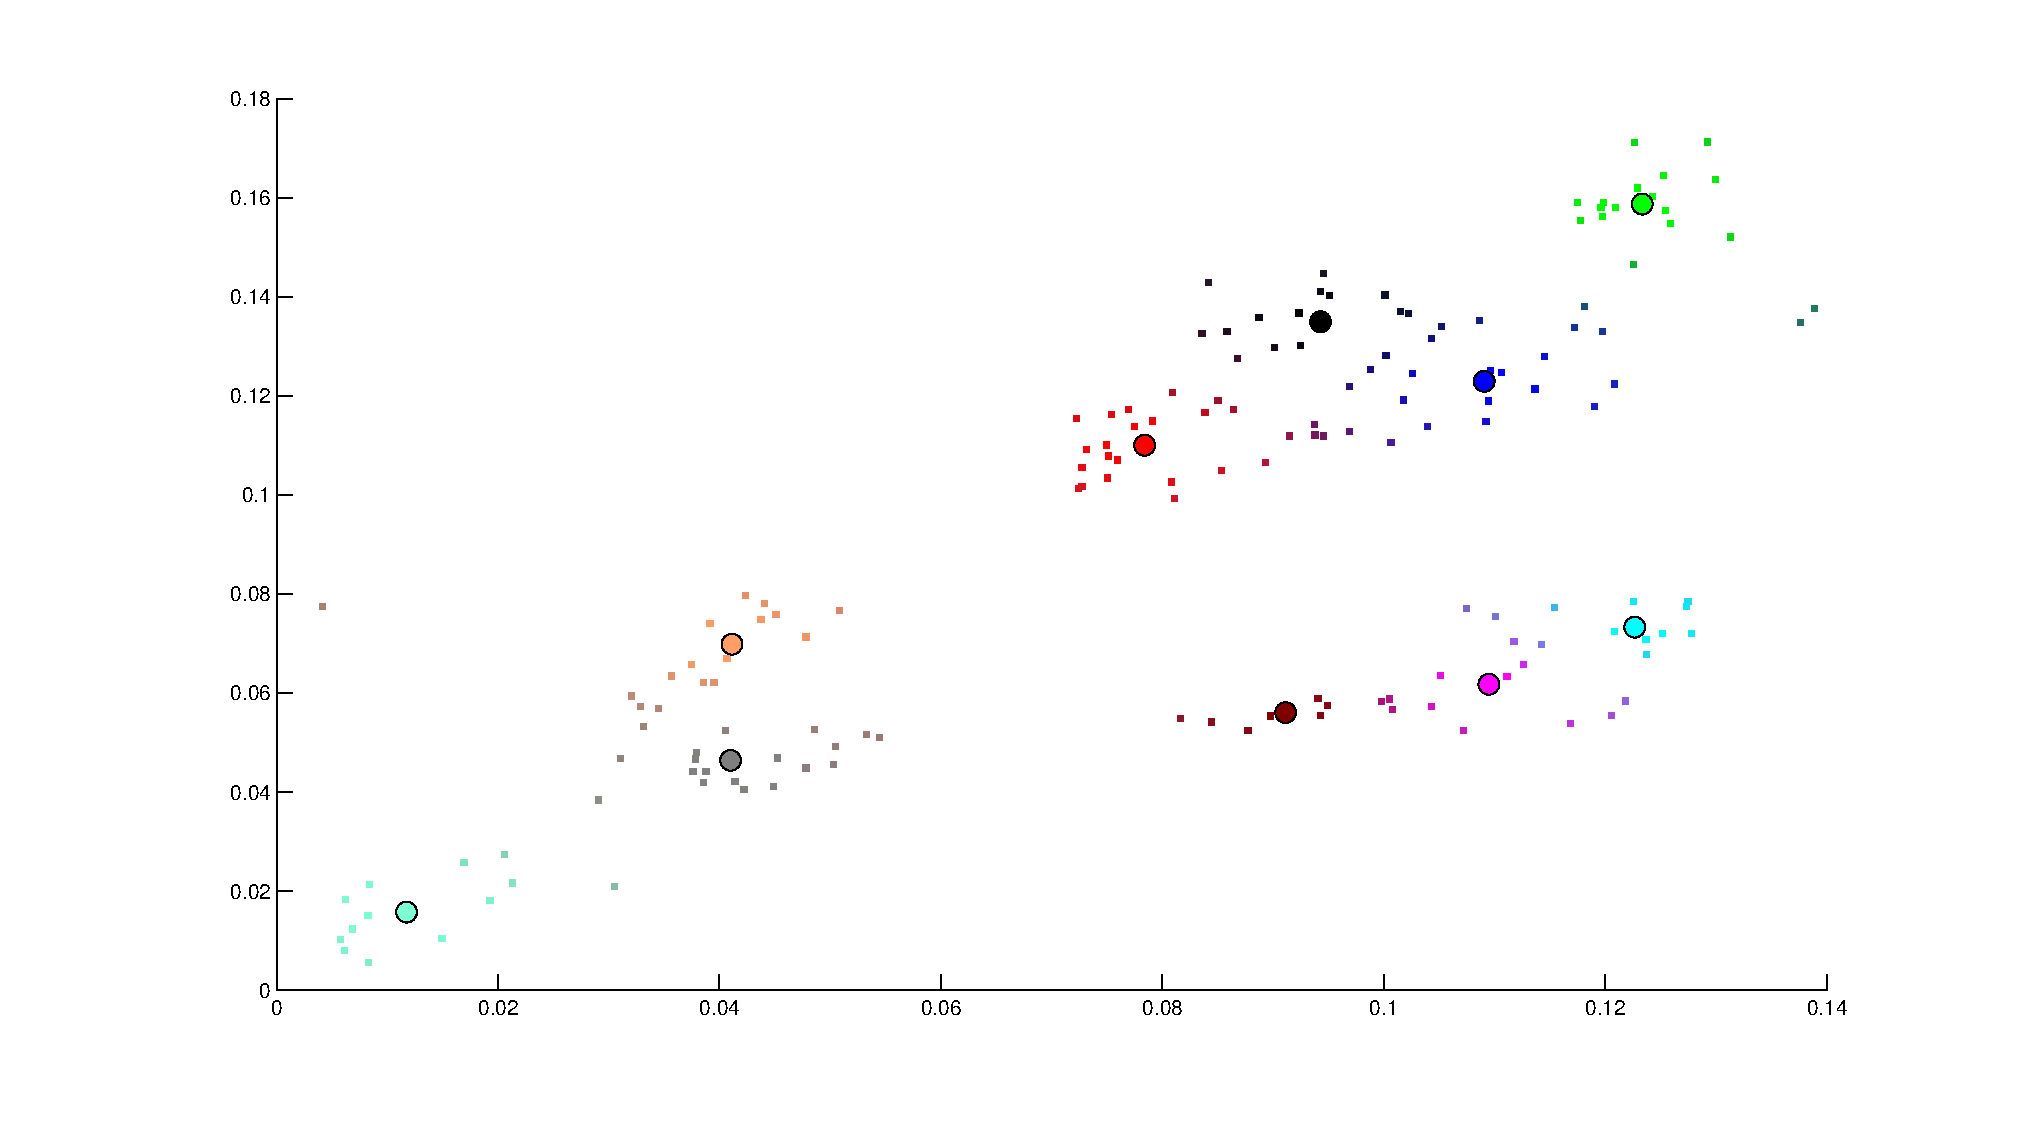
\includegraphics[width=\textwidth]{images/fuzzy-gradient}
\label{fig:k-means-gradientfuzz}
\caption{Prototypes from fuzzy k-means clusters. Data points are
shaded based on probability of belonging to a cluster.}
\end{figure}
